\documentclass{article}
\usepackage{graphicx}
\usepackage{geometry}
\geometry{a4paper, top=2cm, bottom=2cm, left=1.5cm, right=1.5cm}
\graphicspath{{Images/}}
\usepackage{amsthm}
\usepackage{amsmath}
\usepackage{fixltx2e}
\usepackage{xcolor}

\usepackage{verbatim}
\def\SPSB#1#2{\rlap{\textsuperscript{\textcolor{black}{#1}}}\SB{#2}}
\def\SP#1{\textsuperscript{\textcolor{black}{#1}}}
\def\SB#1{\textsubscript{\textcolor{black}{#1}}}
\begin{document}
\newtheorem{definizione}{Definizione}

\tableofcontents
\section{Tokamak}
\subsection{Struttura}
Il Tokamak si basa su tre gruppi elettromagnetici:\begin{itemize}
    \item campo toroidale: funge da manicotto e confina il plasma;
    \item magneti centrale che appartendono al trasformatore e incuono corrente nel plasma che fluisce torodialmente;
    \item magneti del campo verticale: agiscono in modo da stabilizzare il plasma e vincolarlo al centro del toro.
\end{itemize}
\subsection{Confinamento}
Per far avvenire la scarica di plasma, il tokamak deve raggiungere la cosiddetta configurazione di confinamento in cui la risultante del campo magnetico toroidale e poloidale è un campo magnetizo elicoidale: le particelle di plasma si avvitano toroidalmente in superfici isobare di flusso.
\subsection{Scarica}
Durante l'avviamento di un esperimento nel tokamak si inizia crea il vuoto all'interno del vessel e si inietta una miscela di deuterio e trizio all'interno nella camera da vuoto. A questo punto, si innalza il campo toroidale, si ha un ramp up del flusso nel trasformatore per ottenere un alto campo elettrico per poi essere interrotto. Così facendo si crea una differenza di potenziale che avvia un breakdown del plasma: gli elettroni, accelerati dal campo elettrico, guadagnano energia. Questi quando urtano gli atomi di deuterio e trizio lo possono ionizzare e generare un nuovo elettrone. Questo fenomeno si ripete esponenzialmente (avalanche) così da giungere al breakdown del plasma.\newline
Una volta che è trascorso il breakdown viene aviato il controllo in feedback del plasma.
\section{Ruolo delle misure magnetiche}
Le misure magnetiche si possono dividere in due macrocategorie:
\begin{itemize}
    \item \textbf{Operazioni real time}:\begin{enumerate}
        \item \textbf{Posizione del plasma e controllo di forma};
        \item \textbf{Sistema di protezione};
        \item \textbf{Misurazioni};
    \end{enumerate}
    \item \textbf{Analisi offline}:
    \begin{enumerate}
        \item Ricostruzioni magnetiche: superfici di flusso e il bordo del plasma. Sono molto impoortanti per correggere e interpretare le informazioni contenuta in una scarica;
        \item Analisi MHD
    \end{enumerate}
\end{itemize}
\section{Sensori Induttivi}
Il tokamak possiede delle diagnostiche basate su sensori induttivi: sono dei sensori che risentono delle variazioni del campo magnetico in forma integrale o derivativa.\\
I sensori induttivi si basano sulla legge di Faraday: la forza elettromotiva indozza è proporzionale alla derivata del flusso di campo magnetico.\begin{equation}
    fem=-\frac{d \Phi\langle B\rangle }{dt}
\end{equation}
Tuttavia in pratica quello che lo strumento ritorna sono valori di tensione che tramite la relazione:
\begin{equation}
    V=-NA\langle \dot{B}\rangle
\end{equation}
Integrando nel tempo si può avere una misuare del flusso del campo magnetico:\begin{equation}
    \Phi=NA\langle B\rangle =-\int Vdt+const
\end{equation}
Di seguito si illustreranno i sensori induttivi installati in un tokamak.
\subsection{Rogowski Coil}
Le bobine Rogowski sono delle bobine solenoidali che si avvolgono lungo la sezione poloidale del toro. Queste forniscono una misura diretta della corrente che fluisce nel suo centro.\newline L'equazione che la caratterizza è:\begin{equation}
    \Phi = nA \oint B dl \mu_{0}nAI_p=-\int V dt+const
\end{equation}
Bisogna ricordare che:
\begin{itemize}
    \item Le misure di corrente non dipendono sulla forma del rogowski ne dalla distribuzione di corrente nel plasma;
    \item Il cammino degli avvolgimenti del solenoide devono ritornare sullo stesso asse in cui sono iniziate;
    \item Le bobine Rogowski possono essere sostituite da un set di bobine tangenti alla camera.
\end{itemize}
\subsection{Voltage Loop / Flux Loop}
Il Voltage Loop è una singolo cavo che avvolge la camera toroidalmente ed ha il compito di misurare la tensione indotta dal trasformatore centrale. La tensione ai capi della bobina vengono inviato ad un DAS che ne calcola il valore.
\subsection{Pick-Up Coils}
Le Pick-up Coils sono bobine poste al bordo del vessel utilizzare per ricostruisce l'equilibrio, per controllare il plasma e rilevare le instabilità MHD.% chktex 13
\subsection{Saddle Coils}
Le bobine Saddle sono bobine estese montate sulla camera da vuora che permettono di misuare il flusso magnetico perpendicolare a loro stessi. Inoltre, sono utilizzate per la ricostruzione dell'equilibrio e possono fornire in totale misure del flusso poloidale. In quest'ultimo caso, si ottengono misure integrali del flusso poloidale che devono essere derivare con un flusso di riferimento per ottenere una informazione.
\subsection{Loop Diamagnetico}
Sappiamo che il plasma, dall'equazione dell'equilibrio \(j\times B=\nabla p\) le particelle del plasma si dispongono lungo superficie isobare e che l'equilibrio sviluppa delle correnti poloidali che riducono il campo magnetico. Questo specifico comportamento viene detto \textbf{diamagnetismo}.\\
Al fine di misurare l'energia del plasma dal flusso toroidale si utilizza il Loop Diamagnetico. Questa misura risulta non semplice dato che l'effetto diamagnetico è molto piccolo.\newline
Infine, risulta una diagnostica che soffre dell'allineamento.
\subsection{Sensori di Hall}
Una delle problematiche delle diagnostiche a bobine magnetiche è che le misurazioni del campo magnetico rispondono a cambiamenti della derivata del campo magnetico. Ciò implica che in un campo magnetico stazionario queste bobine risultano inutili finché non vengono mosse all'interno del campo.\newline
Per questi tipi di campi si è deciso di introdurre delle diagnostiche che si basasserò sull'effetto Hall.\newline
L'effetto Hall è un fenomeno fisico proprio del plasma in cui si considera il plasma come un semiconduttore solido. In particolare, una lastra di semiconduttore è immersa in un campo magnetico. Una corrente attraversa la lastra e viene affetta dalla forza di Lorentz, deviando perpendicolarmente al prodotto vettoriare tra j e B.\newline
La carica risultante sulle facce della lastra genera un campo elettrico addizionale che cancella la forza magnetica. Quest'ultimo campo elettrico viene misurato dai sensori.
\section{Sistemi di riscaldamento addizionali}
Il principale meccanismo utilizzato nel tokamak per accellerare le particelle è il riscaldamento ohmico. Tuttavia, non è necessario ad accellerare le particelle quanto dovuto dato che questo tipo di risaldamento risulta inefficace ad alte temperature. Questo difetto è dovuto alla resistitività del plasma che diminuisce con l'aumentare della temperatura.\newline
Si necessitano di riscaldamenti addizionali per raggiungere le temperature necessarie. Esse sono basate su riscaldamento da particelle \(\alpha \), su onde elettromagnetiche e su iniezione di particelle neutre.
\subsection{Diagnostiche su atomi neutri} % Grammarly
Le diagnostiche basate su atomi neutri nel plasma sono importanti per plasmi confinati elettromagneticamente poiché essi, essendo neutri, attraversano le linee di campo. Possono essere quindi sfruttati per ottenere delle informazioni sul centro del plasma.\newline
Per creare un fascio neutro si utilizza una miscela da cui si producono gli ioni di deuterio o idrogeno (per maggiore efficienza si sono scelti ioni negativi), a questo punto vengono accellarati da un campo magnetico orizzontale, vengono neutralizzati e poi iniettati all'interno del plasma. Le linee guida per l'iniezione di un fascio neutro sono i seguenti:\begin{itemize}
    \item Le particelle neutre viaggiano inalterate attraverso i campi magnetici;
    \item Il beam trasferisce energia al plasma attraverso le collisioni;
    \item L'assorbimento del fascio deve avvenire al centro del plasma. Se abbiamo fomato un fascio debole allora verrà assorbito nel bordo del plasma; se troppo forte o mal direzionato può bucare la camera da vuoto;
    \item L'assorbimento del fascio dipende dalla sezione d'urto tra il fascio e il plasma;
\end{itemize}
Schematicamente:
\begin{figure}
    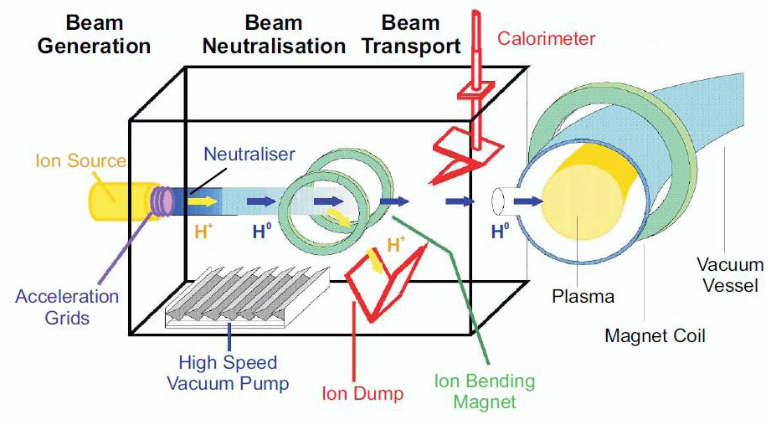
\includegraphics[scale=0.4]{2022-05-17-22-03-45.png}% chktex 8
\end{figure}
\subsection{Electron Cyclotron Resonant Heating}
Le cosiddette ECRH sono riscaldamenti addizionali basati su onde radio per trasferire energia da una sorgente esterna al plasma. Quando una onda elettromagnetica si propaga attraverso il plasma, il campo elettrico dell'onda accellera le particella cariche e quindi aumenta il numero di collisioni di queste nel plasma.\newline
In particolare, si ha assorbimento dell'onda quando si è in risonanza, tuttavia essendo il plasma non uniforme si possono avere anche fenomeni di riflessioni. Ne risulta quindi che la polarizzazione dell'onda gioca un ruolo molto importante sulla forza dell'onda e sulla regione di assorbimento. Vi sono principalmente due distinzioni di polarizzazioni che sono dipendenti dal campo magnetico nel plasma:\begin{itemize}
    \item O-Mode: parallelo al campo magnetico e inconrano solamente una frequenza di risonanza e un di cut-off;
    \item X-Mode: perpendicolare al campo magnetico
\end{itemize}
Un altro fenomeno che potrebbe risentire il fascio è quello della rifrazione quando si trannano plasmi di alta densità.
\section{Thomson Scattering}
Per misurare la temperature e la densità del plasma si sfrutta il fenomeno del Thomson Scattering. In particolare si inietta nel plasma un fascio laser e se ne misura sia la luce diffusa che la larghezza spettrale.\newline
Le misure di larghezza fornisco delle informazioni sulla temperatura e l'intensità della luce diffusa sulla densità degli elettroni. Le ragioni principali per cui si è introdotta questa diagnostica sono due:\begin{itemize}
    \item è un metodo che non perturba l'equilibrio del plasma poiché si richiede solo l'accesso alle radiazioni del plasma;
    \item permette di avere delle informazioni dettagliate sulla funzione di distribuzione degli elettroni.
\end{itemize}
Si ha una onda elettromagnetica incidente su una particella che viene accelerata dai campi elettromagnetici dell'onda. Durante l'urto si ha una emissione di una radiazione detta scattered wave. Questa radiazione viene misurata dagli spettrometri a filtri policromatrici.
Dato che occorre che il posizionamento delle ottiche sia ottimale, la calibrazione diventa fondamentale per ottenere misurazioni della densità di elettroni. Essa viene effettuata utilizzando altri gas.
\section{Polarimetro}

\begin{comment}
    Il polarimetro è necessario per ottenere informazioni sulla densità e corrente di plasma. Si basa principalmente su due fenomeni:\begin{itemize}
    \item Effetto Faraday: nel plasma in presenza del campo magnetico, il piano di polarizzazione del fascio laser propagato nel campo magnetico ruota. Da informazioni su \textbf{Campo magnetico Poloidale};
    \item Effetto Cotton-Mouton: se il fascio laser si propaga perpendicolarmente al campo magnetico vi è un campo dell'ellitticità della polarizzazione.Da informazioni su \textbf{Campo magnetico toroidale}.
\end{itemize}
Il plasma nel campo magnetico si comporta come un mezzo dielettrico con indici di rifrazione diverse in base alle componenti del campo magnetico. In particolare, il pasma è birifrangente e questa proprietà dipende da:\begin{itemize}
    \item Densità elettronica;
    \item Il campo magnetico;
    \item Temperatura elettronica.
\end{itemize}
\begin{definizione}
    Un'onda è detta polarizzata linearmente se la risultante del campo elettrico vibra nella stessa direzione in un particolare punto.
\end{definizione}
La polarizzazione può essere ottenuta da:\begin{itemize}
    \item assorbimento selettivo;
    \item Riflessione;
    \item Scattering;
\end{itemize}
\subsection{Assorbimento Selettivo}
Nell'assorbimento selettivo, un fascio non polarizzato attraversa una lente di polarizzazione che fa passare solo le componenti del campo magnetico su un asse. Poi queste componenti incidono su un analizzatore: il raggio incidente con quello rifratto formerà un angolo che viene misurato.
La particolarità del polarizzatore è che assorbe i vettori di campo elettrico nelle direzioni perpendicolari e trasmette quelle nella direzione parallela.
\subsection{Polarizzazione da doppia rifrazione}
Esistono materiali che possiedono due inidici di rifrazioe differenti. Questi materiali vengono detto birifrangenti.\\
Ne è un esempio la calcite che, quando la luce non polarizzata attraversa il materiale viene divisa in due: raggio straordinario E (varia in base alla direzione di propagazione) e raggio ordinario O (è la stessa lungo tutte le direzioni). Inoltre, vi è una direzione detta \textbf{asse ottico}, su quale i raggi ordinari e straordinari hanno la stessa velocità.
\subsection{Funzionamento}
Supponiamo di avere una onda luminosa che si propaga lungo la direzione z. Sappiamo che questa è una onda elettromagnetica con le componenti del campo magnetico e elettrico perpendicolari l'una dall'altra. Tramite delle funzioni trigonometriche e passaggi algebriche si arriva allìequazione di una ellisse. Quando questo raggio luminoso attraversa il plasma si nota che l'ellisse viene ruotata di un certo angolo
\end{comment}
Il Polarimetro è una diagnostica che consente di avere misure delle componenti del campo magnetico per capire la causa che hanno portato alla rilevazione di tale misure.Queste misure sono fondamentali per la ricostruzione dell'equilibrio del plasma dato che tramite esse è possibile inserire ulteriori vincoli per la risoluzione del problema inverso.\newline
Il funzionamento del Polarimetro si basa su un fascio laser negli infrarossi che fa ad incidere sul plasma. Da questo urto si hanno informazioni riguardo alla corrente di plasma (campo poloidale) e la densità degli elettroni.\newline
L'urto del fascio laser con il plasma, dato che quest'ultimo è un mezzo birifrangente (indice di rifrazione differente in base all'angolo di incidenza del fascio) da origine a due effetti:
\begin{itemize}
    \item Effetto Faraday: il fascio laser ruota, dovuto al campo magnetico poloidale;
    \item Effetto Cotton-Mouton: il fascio laser si ellettifica,dovuto al campo magnetico toroidale;
\end{itemize}
La birifrangenza del plasma dipende da:
\begin{itemize}
    \item densità elettronica;
    \item campo magnetico;temperatura elettronica
\end{itemize}

Il Polarimetro per funzionare ha bisogno di una luce polarizzata: una luca in cui i vettori del campo elettrico non si propagano lungo tutte le direzioni, ma lungo una precisa direzione. Tuttavia, la luce di base non è polarizzata e quindi occrre polarizzarla tramite uno strumento detto polarizzatore.
\subsection{Polarizzatore}
Il polarizzatore è uno strumento che consente di polarizzare la luce non polarizzata. In particolare, data una sorgente di luge non polarizzata, si interpone lungo le direzioni di propagazione della luce un filtro a bande verticale che permette di far passare solo le componenti del campo elettrico parallele alle fenditure del filtro.
In generale la polarrizzazione può essere effettuata tramite:\begin{itemize}
    \item assorbimento;
    \item riflessione;
    \item scattering;
\end{itemize}
\subsubsection{Assorbimento}
L'assorbimento è il metodo più comune per polarizzare la luce. Si necessita di una sorgente di luce non polarizzata, un polarizzatore, un analizzatore hardware capace di valutare l'efficienza del polarizzatore. L'efficienza viene considerata come l'angolo formato tra il raggio incidente e uscente all'analizzatore.
\subsubsection{Polarizzazione tramite doppia rifrazione}
I materiali birifrangenti possono essere utilizzati per la polarizzare la luce. La loro particolarità è che essi posseggono due indici di rifrazione: quando un fascio di luce passa nel materiale birifrangente si genera il raggio straordinario (E) e raggio ordinario (O) dovuto alla diversa velocità di attraversamento del mezzo.\newline
Inoltre, il punto in cui coincidono gli indici di rifrazioni è quello che si trova lungo l'asse del mezzo.
\subsection{Onde elettromagnetiche}
Le onde elettromagnetiche sono composte da componenti perpendicolari fra loro del campo elettrico e magnetico che si propagano lungo una direzione z. Detto ciò possiamo esprimere l'equazioni di un'onda elettromagnetica che si propagna lungo una direzione come:
\begin{equation}
    \overrightarrow{E_{x}}( z,t)=E_{0 x}\cos{(\omega t-kz+\delta_{x})}\overrightarrow{x}\quad \overrightarrow{E_{y}}(z,t)=E_{0 y}\cos{(\omega t-kz+\delta_{y})}\overrightarrow{y}
\end{equation}
Si dimostra che unendo queste due equazioni si giugne all'equazione dell'ellisse dipendendo dalla differenza di fase fra le componenti del campo elettrico dell'onda. A questo punto, data l'equazione dell'ellisse si può calcolare la deformazione del fascio tramite l'ellisse di polarizzazione nel piano \emph{xy}: si individuano gli angoli \(\psi \) di orientamento dell'ellisse e \(\chi \) l'elletticità dal fascio iniziale e quello rifratto.
\subsection{Ellisse di Propagazione e Vettori di Stockes}
L'ellisse di propagazione da cui si ricava l'ellitticità e l'orientamento può essere ricondotta in una forma più semplice tramite i vettori si Stockes. I parametri di Stokes sono un insieme di valori utili a capire se un'onda è polarizzata linearmente, radialmente etc\dots per poi modellizzare il percorso ottico del polarimetro.\newline
In particolare è un vettore composto da 4 componenti dipendenti dall'equazione elettromagnetiche delle onde:\newpage
\begin{figure}[t]
    \centering
    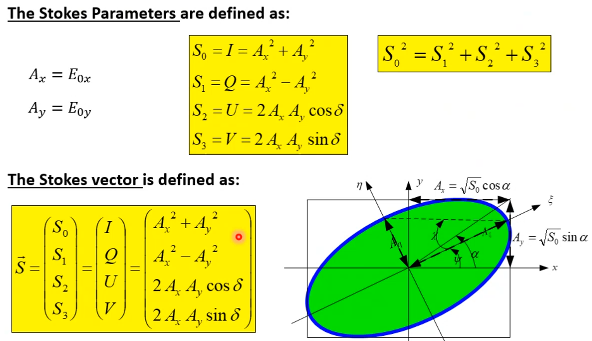
\includegraphics[scale=0.4]{2022-05-24-23-36-23.png}% chktex 8
    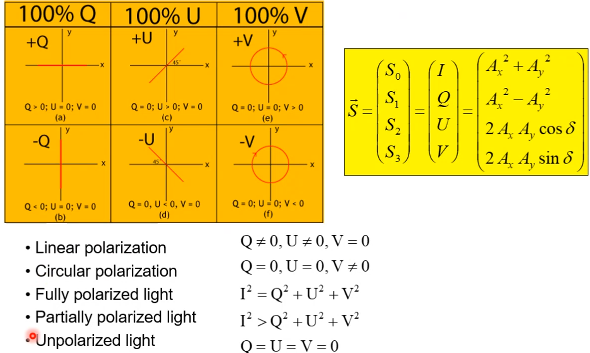
\includegraphics[scale=0.4]{2022-05-24-23-38-37.png}% chktex 8
\end{figure}
Per calcolare l'effetto del Plasma sul fascio laser occorre tenere conto delle componenti ottiche che ha attraversato il fascio laser. Per vedere questo effetto si calcola:
\begin{equation}
    \overrightarrow{S}_{fin}=M_{pol}\cdot \overrightarrow{S}_{in}
\end{equation}
In cui:\begin{itemize}
    \item M:\@matrice che caratterizza il componente ottico;
    \item S in o fin: polarizzazione del fascio iniziale e finale espressi in vettore di Strokes;
\end{itemize}
Ogni elemento ottico viene descritto dalla matrice di Mueller ed è sempre nota.
\subsection{Sistema Polarimetrico}
Gli effetti che entrano in gioco nel polarimetro sono espressi come:
\begin{equation}
    \psi\propto \int n_{e}\cdot B_{z}dz\quad\text{Rotazione di Faraday}
\end{equation}
\begin{equation}
    \phi\propto \int n_{e}\cdot B_{T}^{2}dz\quad \text{Cotton-Mouton}
\end{equation}
L'evoluzione della polarizzazione viene descritta in base alla variazione del vettore di Stokes sull'asse z:
\begin{equation}
    \frac{d\overrightarrow{S}}{dZ}=\overrightarrow{\Omega}\times\overrightarrow{S}
\end{equation}
In cui \(\Omega \) dipende dalla frequenza, dai due indici di rifrazione del mezzo e il vettore di polarizzazione dell'onda veloce. Non ha risoluzione e può essere risolta tramite una matrice simmetrica simile a quella di Muller sia per i componenti ottici che il plasma.\newline
Quindi, per sapere l'effetto che hanno i componenti ottici (inclusi il plasma) si moltiplicano tutte le matrici di Muller come da formula per poi ottenere:
\begin{itemize}
    \item Angolo di rotazione:
    \begin{equation}
    \psi =\frac{1}{2}\arctan{\frac{S_{2}}{S_{1}}}
    \end{equation}
    \item Cotton-Mouton: \begin{equation}
        \arctan{\frac{S_{3}}{S_{2}}}
    \end{equation}
\end{itemize}
\section{MSE}
L'MSE è una diagnostica che permette di avere delle misure interne al plasma tramite un'analisi degli atomi neutri.\newline
Dato che gli atomi immessi sono neutri non interagiscono con i campi magnetici, ma possono interagire con gli atomi del plasmi così da inferire a delle proprietà del plasma. L'immissione del fascio neutro è anche un sistema di riscaldamento nel NBI.% chktex 13
\subsection{Motion Stark Effect}
L'MSE è una diagnostica che utilizza la luce che proviene dai NBI ad idrogneo (utilizzati per il riscaldamento addizinaale) e l'interazione con il plasma. La luce proveniente dall'idrogeno eccitato uò essere osservato all'interno della lunghezza d'onda di Balmer \(\alpha \): la luce emessa è polarizzata e la sua banda risulterà allargata a causa del campo magnetico.
\subsection{Principi NBI}
\begin{itemize}
    \item Le particelle neutre viaggiano inalterate attraverso i campi magnetici;
    \item Il beam trasferisce l'energia al plasma tramite le collisioni;
    \item L'assorbimento del beam deve avvenire al centro e non al bordo e questo è dovuto alla potenza del fascio;
    \item I processi principlai sono:\begin{figure}
        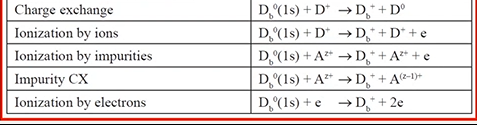
\includegraphics[scale=0.4]{2022-05-26-23-49-28.png}%chktex 8
    \end{figure}
\end{itemize}
\subsection{Spettroscopia}
Come abbiamo visto l'MSE si basa sullo spettro della luce emessa dall'interazione del fascio con il plasma.\newline
Lo spettrometro misura per varie lunghezze d'onda la luce emessa dall'idrogeno. Le varie bande sono dovuto allo shift doppler. Questo fenomeno è vantaggiso poiché permette di distinguere tra le emissioni dell'idrogeno e quelle al bordo.\newline In particolare, l'informazione è contenuta nell'intensità della linea: più è intensa più il plasma è denso in una determinata porzione di plasma. Un altro modo per vedere lo spettrogramma è quello di utilizzare i fasci quantici: l'energia emessa dipende dalla costante di Planck e la frequenza della luce emessa.
\subsection{Stark Effect}
L'effetto Stark è quell'effetto che quantifica la separazione delle bande dello spettro dell'idrogeno in presenza di un campo elettrico. (Nel caso in cui si parlasse di campo magnetico si chiama Effetto Zeeman).\newline
Vedendo uno spettrometro, si vedono più picchi e degli allargamenti delle bande: l'aggiunta dei picchi sono dovuto all'energia con cui entrano i NBI nel plasma che va a diminuire a \(\frac{1}{i}\quad u=1,..,n\). Inoltre, si nota una variazione della lunghezza d'onda della luce è dovuto all'effetto Doppler: il cambio della lunghezza d'onda della radiazione è dovuta al moto relativo tra sorgente e osservatore. Si quantifica:
\begin{equation}
    \frac{\Delta\lambda}{\lambda_{0}}=\frac{v}{c}
\end{equation}
\subsection{Motional Stark Effect}
Il contributo dominante per la struttura spettrale di un componente monoenergetico del fascio è dovuto al motional Stark Effect. Questo effetto non è differente dal classico Stark Effect, ma il campo elettrico in question non è vicino al plasma. Tuttavia, sorge dal movimento dell'atomo all'interno del campo magnetico, ma risentirà di un campo elettrico dovuto alla forza di Lorenzt.\newline
Il suo effetto può essere di due tipo:\begin{itemize}
    \item Quadratico: si ha quando si considera il momento della carica;
    \item Lineare
\end{itemize}
Lo stark effect si compone di due regimi:\begin{itemize}
    \item Per la maggioranza degli aotmi lo stark effect è quadratico in particolare rispetto al campo elettrico. Questo perché il momento del dipolo elettrico dell'atomo è proporzionale all'applicazione del campo e all'energia della perturbazione.
    \item Lineare: quando si è in presenza di campi elettrici forti in cui questa energia è comparaile alla divisione dello spettro dei livelli di energia (numero quantico) di un atomo non perturbato. Le barre si dividono in barre sigma e pi greco nella serie di balmer in cui la loro altezza rappresenta l'intensità dello spettro e si differenziano in polarizzazione.In particolare:\begin{itemize}
        \item La componente \(\pi \) relativo al numero quantico 0 risulta in un'onda polarizzata nella componente parallela del campo elettrico;
        \item La componente \(\sigma \) con numero quantico pari a +/- 1 alla componente perpendicolare del campo elettrico
    \end{itemize}
\end{itemize}
\section{Interferometro}
L'interferometro è una diagnostica che consente di misurare la densità del plasma. Ancque questa diagnostica come il polarimetro si basa sulle ottiche.\newpage
\subsection{Onde ottiche}
Quando si trattano le onde si possono verificare 3 tipi di eventi:\begin{itemize}
    \item Interferenza;
    \item Diffrazione: se il fascio laser passa tramite due fenditure, si nota che al passaggio delle fenditure disegna delle figure di diffrazione corrispondente ad una dispersione dell'onda;
    \item Polarizzazione.
\end{itemize}
Affinché sia possibile verificars di questi eventi necessitiamo che il fascio sia:\begin{itemize}
    \item Coerente: deve mantenere una fase costante;
    \item Monocromatica: il laser deve avere una singola lunghezza d'onda.
\end{itemize}
\subsection{Interferenza}
Date due sorgenti coerenti e monocromatiche esse possono interagire in due maniere:\begin{itemize}
    \item Costruttuiva: se l'ampiezza dell'onda risultante è maggiore di quella singola;
    \item Distruttive: se l'ampiezza dell'onda risultante è meno di una delle due sorgenti.
\end{itemize}
Tutte le interferenza associate ai fasci di luce sono associate all'interazione dei campi elettromagnetiche. Visivamente, in un interferometro, il fenomeno di interferenza origina una sequenza di bande chiare e scure corrispondenti rispettivamente a fenomeni di interferenza costruttiva e distruttiva. Queste bande sono ottenute da uno schermo posto ad una certa distanza dalle fenditure: le onde delle due sorgenti corrispondenti alle due fenditure formano una interferenza costruttiva se le onde arrivano sullo schermo in fase (una onda corre più dell'altra) e altrimenti è distruttiva.
In formule:\begin{itemize}
    \item Interferenza costruttiva: \(\delta= d\sin{(\theta_{\text{brigth}})}=m\lambda \)
    \item Interferenza distruttiva  \(\delta= d\sin{(\theta_{\text{dark}})}=(m+\frac{1}{2})\lambda \)
\end{itemize}
Da cui possiamo calcolare la posizione delle frange:\begin{itemize}
    \item \(y_{\text{k}}=L\tan{\theta_{\text{k}}}\quad k =\{\text{brigth,dark}\} \)
\end{itemize}
Inoltre, assumendo che la distanza fra gli schermi è molto più grande della distanza tra le fenditure e quest'ultima è molto più grande della lunghezza d'onda si sostituisce la tangente con il seno (condizione di piccolo angolo) che è noto. Così facendo, si ottiene una formula che non dipende dall'angolo:\begin{equation}
    y_{\text{brigth}}= L\frac{m\lambda}{d}\quad  y_{\text{dark}}= L\frac{(m+\frac{1}{2})\lambda}{d}
\end{equation}
Ottenuta la posizione, ora vogliamo caratterizzare l'ampiezza dell'intensità luminosa corrispondente alla frangia rilevata sullo schermo. Dalle equazioni dell'onda:\begin{align}
    E_{1}&=E_{0}\sin{\omega t}\\
    E_{2}&=E_{0}\sin{\omega t+\phi}
\end{align}
Dal principio di sovrapposizione degli effetti si ottiene:\begin{equation}
    E_{p}=2E_{0}\cos{\frac{\phi}{2}}\sin{\omega+\frac{\phi}{2}}
\end{equation}
La differenza di fase tra le due onde nel punto P dello schermo è:\begin{equation}
    \delta=r_{1}-r_{2}=d\sin{\theta}
\end{equation}
con r percorso generato tra le due fenditure.
Si può scrivere l'intensità dell'onda sarà proporzionale al quadrato della risultante dell'intensità del campo elettrico. Graficamente:\begin{itemize}
    \item L'interferenza consiste in bande equispaziate di uguuale intensita.
    \item Nei picchi interferenza costruttiva;
    \item Nelle valli interferenza distruttiva.
\end{itemize}
\subsection{Diagnostiche}
Vi sono due possibili configurazioni di diagnostiche utilizzano l'interferenza:\begin{itemize}
    \item Michelson;
    \item Mac-Zender;
\end{itemize}
\subsubsection{Interferometro di Michelson}
La sorgente di luce incide su un bisplitter che dividerà il fascio in due. Entrambi i fasci laser attraversando il bisplitter incidono su due specchi M1,M2 posti a distanza L1 e L2 e uno specchio si trova a 90 gradi della sorgente, l'altro parallelamente alla sorgente.\newline
I due rami riflessi dagli specchi ritornano indietro sul bisplitter e vengono osservati. Ricomponendosi, si ottengono le immagini di interferenza in base alla distanza degli specchi del bisplitter.
\begin{figure}
    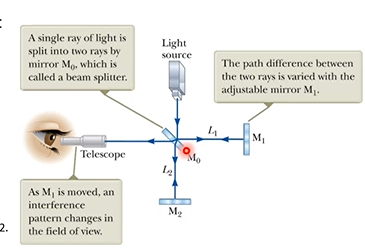
\includegraphics[scale=0.4]{2022-05-29-15-59-34.png}% chktex 8
\end{figure}
Il vantaggio di questo strumento è che non si necessita di calibrazione dato che la misura che viene acquisita è una misura relativa tra i bracci degli specchi: la sorgente è la stessa e viene divisa da un componente ottico (a patto che le ottiche non si siano guastate).
\subsection{Interferometro nella fusione}
L'interferometro utilizza dei fasci a frequenze molto lontane da quelle del plasma così da non perturbarlo ed avere delle misure ottimali sulla densità di plasma e insieme al polarimetro sulle componenti del campo magnetico.\newline
I vantaggi di questa diagnostica sono i seguenti:\begin{itemize}
    \item Si segue l'evoluzione del plasma istante per istante sulla densità degli elettroni;
    \item Non si necessita di calibrazione per gli strumenti;
    \item Non si necessitano di informazioni addizionali da altre diagnostiche.
\end{itemize}
\subsubsection{Mach-Zender}
 \begin{figure}
     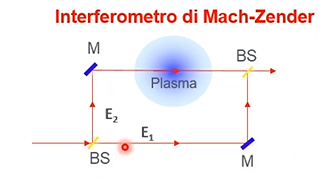
\includegraphics[scale=0.4]{2022-05-29-16-10-11.png}% chktex 8
 \end{figure}
 Si ha il fascio laser che viene diviso da un bisplitter: un ramo passa per il plasma e l'altro no. In seguito ripassano per un altro bisplitter per essere ricomposte ed analizzate. Questa configurazione è detta autocalibrante poiché si prende sempre il segnale di riferimento dal fascio che non passa per il plasma.
 \begin{figure}
     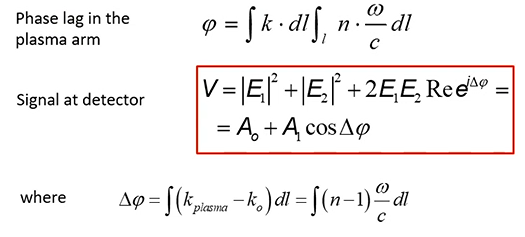
\includegraphics[scale=0.4]{2022-05-29-16-13-05.png}% chktex 8
 \end{figure}
 Il parametro \(n\) di rifrazione del plasma può essere scritta come:\begin{equation}
     n^{2}=\frac{n_{e}}{n_{c}}
 \end{equation}
 La frequenza del plasma dipende da:\begin{itemize}
     \item Densità elettronica;
     \item Constante dielettrica nel vuoto;
     \item Carica elettronica;
     \item Massa dell'elettrone;
 \end{itemize}
 Per una frequenza fissata si definisce la densità di cut-off come la densità per cui la frequenza del fascio laser è uguale alla frequenza di plasma. Se la densità eccede il valore di cutoff, l'onda non è più propagata, ma decade esponenzialmente con la distanza. Ciò risulta che normalmente si trasmette una piccola potenza attraverso il plasma e l'interferometro cessa di funzionare.
 \subsubsection{Interferometro nel JET}
 \begin{figure}
     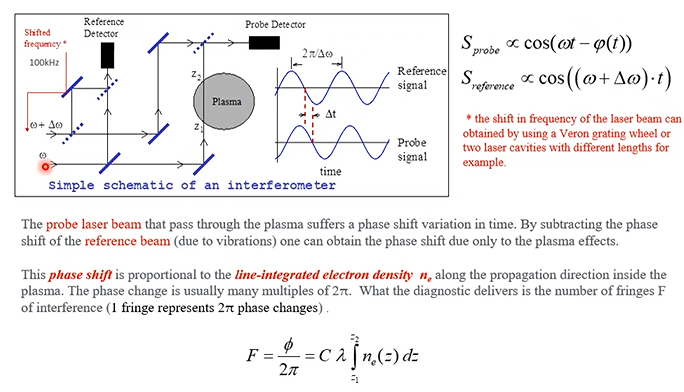
\includegraphics[scale=0.4]{2022-05-29-16-23-12.png}% chktex 8
 \end{figure}
 \subsection{Problemi dell'interferometro: salti di frangia}
 Le misure interferometriche possono perdere il segnale quando l'onda del fascio è un multiplo elevato del plasma e quindi si perdono le misurazioni della densità del plasma. Per ovviare a questo problema o si ferma la scarica o si continua lo sparo e poi si avvia la fase di ricostruzione del segnale. Tuttavia, il metodo più efficiente è quello di utilizzare il polarimetro per fittare i dati sull'interferometro.
 \section{Hardware}
\begin{itemize}
    \item Lunghezza d'onda: componente principale da cui dipende la scelta di tutte le altre componentistiche:\begin{itemize}
        \item Onda lunga:\begin{itemize}
            \item Pro:Migliore risoluzione delle misure;
            \item Contro: rifrazione;
        \end{itemize}
        \item Onde corte:\begin{itemize}
            \item Pro: bassa rifrazione;
            \item Contro: Problemi di vibrazioni meccaniche e bassa risoluzione.
        \end{itemize}
    \end{itemize};
    \item Laser: il laser opera nel lontano infrarosso. Devono essere stabili poiché molti laser dipendono dalle condizioni ambientali nel quale operano. Per essere sicuri della stabilità dello strumento si isolano gli strumenti in condizioni ambientali ottimali con un controllo in feedback;
    \item Ottiche le componenti ottiche devono lavorare in ambienti ad alte temperature, radiazioni e neutroni. Quindi bisogna scegliere i materiali con cui sono relizzate le ottiche avento particolare cura a scegliere dei materiali che non risentono dei campi magnetici;
    \item Modulatori\begin{figure}
        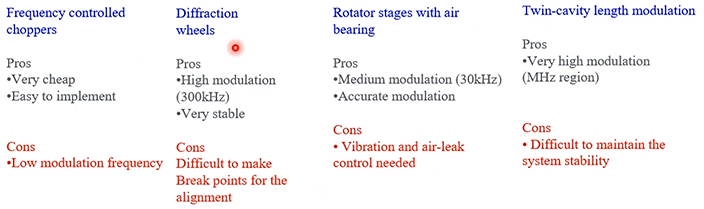
\includegraphics[scale=0.4]{2022-05-29-16-41-03.png}% chktex 8
    \end{figure};
    \item Rivelatori:\begin{figure}
        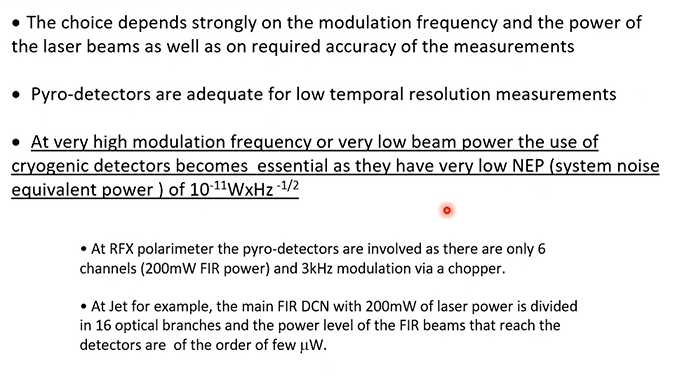
\includegraphics[scale=0.4]{2022-05-29-16-41-40.png}% chktex 8
    \end{figure};
    \item Struttura meccanica;
    \item Controllo dell'atmosfera.
\end{itemize}
\section{Neutronica 1-2-3-4}% chktex 8
\subsection{Introduzione}
\begin{itemize}
    \item \textbf{Struttura Nucleare}:\begin{itemize}
        \item \textbf{Nucleone}: è il nome dato alla particella \SPSB{A}{Z}X
        \item \textbf{Nuclide}: è una paricolare compinazione di protoni e neutroni che compongono un nucleo. Vengono usati per distinguire gli isotopi tra i nuclei.
        \item \textbf{Numero di nucleoni}: Il numero di nucleoni A coincide con il umero di massa ed è definito come la somma dei protoni e dei neutroni nel nucleo. Viene misurato in unità di massa atomica u.
        \item \textbf{Numero di protoni}: Z è il numero dei protoni nel nucleo;
        \item \textbf{Isotopi}: Un istopi sono nuclei con lo stesso numero di protoni, ma differente numero di neutroni. Tramite A e Z si riconoscono i vari tipi di isotopi;
        \item \textbf{Numero di neutroni}: N=A-Z è il numero di neutroni nel nucleo;
    \end{itemize}
    \item\textbf{Isotopi}:Un isotopo è atomo con stesso numero di protoni, ma differente numero di neutroni. L'esistenza degli isotopi è una conseguenza dell'esistenza dei neutroni: non vi è un'altra spiegazione per spiegare la differenza di massa fra due isotopi dello stesso elemento. Dato che le masse differiscono, allora si hanno diverse proprietà fisiche.\newline
    Per l'idrogeno vi sono 3 tipi di isotopi: prozio (stabile), deuterio (stabile) e trizio (instabile, radioattivo). Quelli utilizzati nella fusione sono deuterio e trizio. Il trizio non è molto presente in natura poiché decade velocemente quindi in un Tokamak occorre produrlo artificialmente;
   
\end{itemize}
\section{Tomografia}
\section{Bolometria}
\section{Spettroscopia}
\section{Disruzioni}
Le disruzioni nei Tokamak sono inevitabili. Esse sono una perdita globale di confinamento e controllo del plasma dovuto da impurezze e radiazioni.\newline
Si compongono di due fasi:
\begin{itemize}
    \item Termal quence: perdita di tutta l'energia cinetica e termica;
    \item Current quence: decadimento di corrente
\end{itemize}
In particolare, si ha una fase lontana dalla disruzione non si ha un indizio della disruzione. Dopo di che, si ha un segnale di precorso nelle bobine magnetiche che indica l'inizio di una anomalia. Passata questa fase, si hanno delle anomalie sul profilo di temperatura e corrente così da innescare il termal quence e quindi l'inizio di una disruzione, perdendo di conseguenza il controllo.\newline
Il problema principale di questo fenomeno è che avvenuta la disruzione si danneggiano i dispositivi e si introducono impurezze nel vessel che diminuiscono il tempo operativo del Tokamak. I danni principali sono:
\begin{itemize}
    \item Carichi termici;
    \item Estinzione della corrente rapida porta a carichi magnetici molto elevati dovuto alle correnti indotte (Eddy current);
    \item Elettroni di runaway nella fase di current quenche: in questa fase il plasma perde la densità, così vengono accellarati notevolmente divenendo un fascio di elettroni incontrollato in assenza di collisioni per limitarne la velocità.
\end{itemize}
\subsection{Classificazione diagnostiche disruzione}
L'obiettivo delle diagnostiche per le disruzioni è quello di predizioni, spiegazione e controllo. Si dividono in:
\begin{itemize}
    \item monitorazione delle conseguenze;
    \item misura della disruzione;
    \item investigazione della fisica della disruzione;
    \item predizione delle disruzione
\end{itemize}
Queste diagnostiche fanno parte del sistema di controllo e quindi è necessario che l'hardware siano affidabili, disponibili, forniscano un risoluzione spaziale e temporale per prevenire il fenomeno e devono coprire tutti i punti della camera da vuoto. Inoltre, al livello di processamento deve essere in real-time ed avere capacità predittive.
Una scarica disruttiva presenta la seguente nomenclatura:
\begin{itemize}
    \item Avoidance: la fase lontana di disruzione;
    \item Prevenzione: azione correttiva per evitare l'instabilità;
    \item Mitigazione: nel caso in cui la prevenzione non è abbastanza d avviene la disruzione si riducono i carichi abbassando lentamente la corrente e l'energia termica. In questo fase possono avvenire i run-away. Si immettono pellet di gas per ridurre il carico termico o degli shattered pellet.
\end{itemize}
\subsection{Requisiti Hardware}
\subsubsection{Carichi termici}
Il problema principale sono i carichi termici che dipendono dalla potenza deposita, dalla superfice e dal tempo. Le misure che si utilizzano sono:\begin{itemize}
    \item Camere termiche;
    \item Spettrometria;
    \item Bolometria
\end{itemize}
La problematica di queste misure è che il carico termico non sono toroidalmente simmetrici.
\subsubsection{Carichi Meccanici}
Le misure che si utilizza sono:\begin{itemize}
    \item bobine in posizioni differenti per eseguire una ricostruzione dell'equilibrio;
    \item Misure delle correnti toroidali del vessel (Halo currents);
    \item Accelerometria per misurare gli spostamenti della camera da vuoto
\end{itemize}
\subsection{Locked mode detection AUG}
Siamo nella fase di mitigazioni per cui dobbiamo predirre con un margine di predizioni basso, ma molto accurato.\newline
In questa fase, vi sono delle instabilità MHD macroscopiche con misure magnetiche grande. La crescita delle istabilità vengono misurate con la componente radiale del campo magnetico tramite le Saddle Coils. In un tokamak ve ne sono 4 e tramite la differenza di queste bobine opposte e tramite un indicatore si misura l'effetto di rallentamento delle instabilità. Esse crescono nella fase preliminare della disruzioni, poi rallentano fino a zero e poi disrompe. Viene detto bloccato poiché il campo magnetico da loro generato si blocca con gli errori del Tokamak divenendo stazionari nel sistema di riferimento del laboratorio.\newline
Analizzando lo spettro a bassa frequenza si nota che le instabilità MHD non sono le uniche fautrici delle disruzioni, ma anche dovute dai cosiddetti ELMS.% chktex 13
\subsection{Imaging for disruptions}
Si utilizzano delle telecamere nel visibile per avere una idea di quello che accade nella camera da vuoto. Risulta quindi molto importante cercare di ricoprire il maggiorspazio dellla camera da vuoto e del vessel. Tramite queste telecamere è possibile rivelare i MARFE.\newline
I MARFE sono instabilità termiche che si manifestano come un anello di radiazioni visibili per effetto delle impurezze. In queste zone la temperatura risulta più bassa rispetto al plasma.
\subsection{Indicatori di Profilo}
Per la predizione delle disruzione e il controllo in feedback sono necessari gli indicatori di profilo.\\ GLi indicatori di profilo per la predizione devono essere robusti e calcolabili in real time, ma allo stesso tempo devono fornire  un quantitativo sufficiente di informazioni. Uno degli indicatori sul profilo di temperatura è la hollowness cioè quanto il profilo di temperatura è cavo. Questa è una misura particolarmente difficile da quantificare dato che in molti casi si deve effettuare il mirroring dei dati sull'asse magnetico per un problema di coverage e che è resiliente sulle fluttuazioni della temperatura.\newline
Per questa misura si utilizza un fitting basato su due Gaussiane quando il profilo è cavo: differenze tra i due massimi e normalizzata per la deviazione standard delle  gaussiane. Con questo approccio, più due massimi sono distanti più il profilo sarà cavo.
\subsection{Problema inverso nella fusione}
Per quanto riguardo le misure effettuate dall'esterno del plasma, esse vengono utilizzate nella risoluzione di un problema inverso per ottenere delle informazioni dell'interno. Il principale strumento che viene utilizzato è la tomografia.
Da aggiungere disruzioni 2
\section{Machine Learning}
\end{document}